\documentclass{beamer}
\usepackage[utf8]{inputenc}
  
\usetheme{Madrid}
\usecolortheme{default}
\usepackage{amsmath,amssymb,amsfonts,amsthm}
\usepackage{txfonts}
\usepackage{tkz-euclide}
\usepackage{listings}
\usepackage{adjustbox}
\usepackage{array}
\usepackage{tabularx}
\usepackage{gvv}
\usepackage{lmodern}
\usepackage{circuitikz}
\usepackage{tikz}
\usepackage{graphicx}
\usepackage[T1]{fontenc}
\UseRawInputEncoding

\setbeamertemplate{page number in head/foot}[totalframenumber]

\usepackage{tcolorbox}
\tcbuselibrary{minted,breakable,xparse,skins}



\definecolor{bg}{gray}{0.95}
\DeclareTCBListing{mintedbox}{O{}m!O{}}{%
  breakable=true,
  listing engine=minted,
  listing only,
  minted language=#2,
  minted style=default,
  minted options={%
    linenos,
    gobble=0,
    breaklines=true,
    breakafter=,,
    fontsize=\small,
    numbersep=8pt,
    #1},
  boxsep=0pt,
  left skip=0pt,
  right skip=0pt,
  left=25pt,
  right=0pt,
  top=3pt,
  bottom=3pt,
  arc=5pt,
  leftrule=0pt,
  rightrule=0pt,
  bottomrule=2pt,
  toprule=2pt,
  colback=bg,
  colframe=orange!70,
  enhanced,
  overlay={%
    \begin{tcbclipinterior}
    \fill[orange!20!white] (frame.south west) rectangle ([xshift=20pt]frame.north west);
    \end{tcbclipinterior}},
  #3,
}
\lstset{
    language=C,
    basicstyle=\ttfamily\small,
    keywordstyle=\color{blue},
    stringstyle=\color{orange},
    commentstyle=\color{green!60!black},
    numbers=left,
    numberstyle=\tiny\color{gray},
    breaklines=true,
    showstringspaces=false,
}



\title 
{MatGeo Assignment 4.13.76}

\author
{AI25BTECH11007}
\begin{document}

\frame{\titlepage}
\begin{frame}{Question}
Two lines

\[
L_1 : \frac{x}{5} \;=\; \frac{y}{3-\alpha} \;=\; \frac{z}{-2}
\]

\[
L_2 : \frac{x}{\alpha} \;=\; \frac{y}{-1} \;=\; \frac{z}{2-\alpha}
\]

are coplanar. Then the value(s) of \(\alpha\)
\end{frame}

\begin{frame}{Solution}
    \[
L_1 : \frac{x}{5}=\frac{y}{3-\alpha}=\frac{z}{-2},\qquad
L_2 : \frac{x}{\alpha}=\frac{y}{-1}=\frac{z}{2-\alpha}.
\]

\[
\text {Direction vectors are :   } 
\mathbf n_1=\myvec{5\\[2pt]3-\alpha\\[2pt]-2},\qquad
\mathbf n_2=\myvec{\alpha\\[2pt]-1\\[2pt]2-\alpha}.
\]

\[
\text{Choose points on each line, as both lines pass through the origin, so, }\\
\mathbf p_1=\mathbf p_2=\myvec{0\\0\\0}.
\]

Two lines are coplanar iff
\[
\operatorname{rank}\big(\, \myvec{\mathbf n_1 & \mathbf n_2 & \mathbf p_2-\mathbf p_1}\,\big)\le 2.
\]
\end{frame}
\begin{frame}
Here \(\mathbf p_2-\mathbf p_1=\myvec{0\\0\\0}\), so the matrix becomes
\[
\myvec{5 & \alpha & 0\\[2pt] 3-\alpha & -1 & 0\\[2pt] -2 & 2-\alpha & 0},
\]
whose rank is at most \(2\) for every \(\alpha\). Hence the two lines are coplanar for all real \(\alpha\).

\[
\boxed{\alpha\in\mathbb R}
\]

\end{frame}

\begin{frame}{Plot}
    \begin{figure}
        \centering
        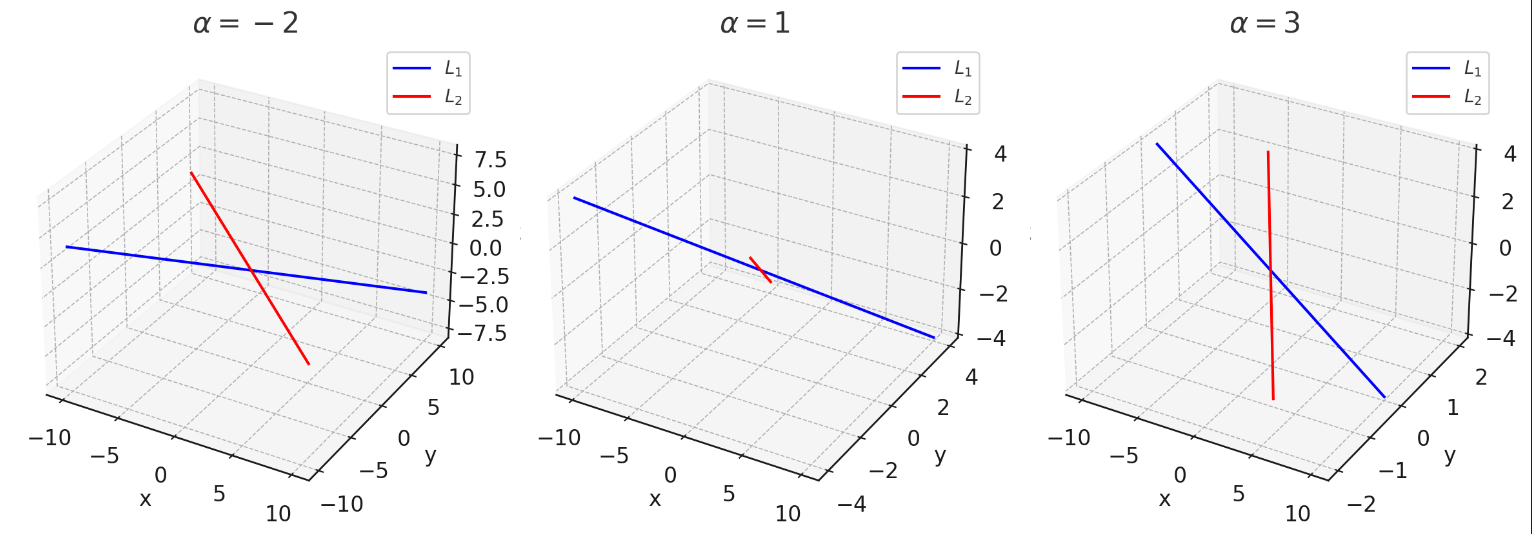
\includegraphics[width=1\linewidth]{figs/image.png}
        \caption{Image}
        \label{fig:placeholder}
    \end{figure}
\end{frame}

\begin{frame}[fragile]{C code}
\begin{lstlisting}
#include <stdio.h>

// Function to compute determinant of 3x2 augmented with 0 column
// Actually we compute rank check: det([n1 n2]) = 0 always
int main() {
    int alpha;
    printf("Lines:\n");
    printf("L1: x/5 = y/(3-alpha) = z/(-2)\n");
    printf("L2: x/alpha = y/(-1) = z/(2-alpha)\n\n");

    printf("Checking coplanarity for sample alpha values...\n");

    for(alpha = -3; alpha <= 5; alpha++) {
        int n1[3] = {5, 3 - alpha, -2};
        int n2[3] = {alpha, -1, 2 - alpha};
\end{lstlisting}
\end{frame}

\begin{frame}[fragile]{C code}
\begin{lstlisting}
    // Compute determinant of 3x2 matrix (v1, v2)
        // In coplanarity test: rank <= 2 always (since both pass through origin)
        // Let's check cross product
        int cross[3];
        cross[0] = n1[1]*n2[2] - n1[2]*n2[1];
        cross[1] = n1[2]*n2[0] - n1[0]*n2[2];
        cross[2] = n1[0]*n2[1] - n1[1]*n2[0];

        printf("alpha = %d -> Lines are coplanar (always true)\n", alpha);
    }

    printf("\nConclusion: Lines are coplanar for all real alpha.\n");
    return 0;
}
\end{lstlisting}
\end{frame}

\begin{frame}[fragile]{Python code}
\begin{lstlisting}
    import numpy as np

def check_coplanarity(alpha):
    # Direction vectors
    v1 = np.array([5, 3 - alpha, -2])
    v2 = np.array([alpha, -1, 2 - alpha])

    # Form matrix with direction vectors as columns
    M = np.column_stack((v1, v2))

    # Rank of coefficient matrix
    rank = np.linalg.matrix_rank(M)

    # Since both lines pass through origin, always coplanar
    return rank <= 2
\end{lstlisting}
\end{frame}

\begin{frame}[fragile]{Python code}
    \begin{lstlisting}
       # Test for some sample alpha values
alpha_values = [-3, -1, 0, 1, 2, 3, 5]
for a in alpha_values:
    result = check_coplanarity(a)
    print(f"alpha = {a:2d} -> Coplanar: {result}")

print("\nConclusion: Lines are coplanar for all real alpha.") 
    \end{lstlisting}
\end{frame}

\end{document}

